\documentclass[11pt, aspectratio=16:9]{beamer}

% Theme and color scheme
\usetheme{Madrid}
\usecolortheme{beaver}

% Packages
\usepackage[utf8]{inputenc}
\usepackage{listings}
\usepackage{xcolor}
\usepackage{tikz}
\usepackage{booktabs}
\usetikzlibrary{arrows.meta, positioning, shapes.geometric}

% Code highlighting setup
\lstset{
    basicstyle=\ttfamily\small,
    breaklines=true,
    keywordstyle=\color{blue},
    commentstyle=\color{gray},
    stringstyle=\color{red},
    showstringspaces=false,
    frame=single,
    backgroundcolor=\color{gray!10}
}

% Custom colors
\definecolor{checkcolor}{RGB}{0,128,0}
\definecolor{crosscolor}{RGB}{200,0,0}

% Document metadata
\title{Working Effectively with AI in Software Development}
\subtitle{Mental Models, Patterns, and Practical Workflows}
\author{Your Name}
\institute{Your Organization}
\date{\today}

\begin{document}

% ===================================================================
% TITLE SLIDE
% ===================================================================
\begin{frame}
\titlepage
\vfill
\centering
\small{Duration: 1.5 hours (40 min presentation + 50 min demo + discussion)}
\end{frame}

% ===================================================================
% OPENING SECTION
% ===================================================================

\begin{frame}{You're Already Using AI}
\large
You're likely already using AI for:

\begin{itemize}
    \item Autocomplete suggestions while typing
    \item Answering questions about APIs and syntax
    \item Generating boilerplate code
    \item Explaining errors
\end{itemize}

\vspace{1em}

\begin{alertblock}{Today's Goal}
\textbf{Most developers already use AI every day.} This session is about being more systematic and intentional about it—extracting maximum value while avoiding common pitfalls.
\end{alertblock}
\end{frame}

% ===================================================================
% FOUNDATIONS SECTION
% ===================================================================

\section{Foundations}

\begin{frame}{How Language Models Work: Tokens}
\begin{columns}[T]
\column{0.48\textwidth}
\textbf{What they are:}
\begin{itemize}
    \item Text broken into chunks
    \item Model processes tokens sequentially
    \item Generates output one token at a time
\end{itemize}

\column{0.48\textwidth}
\textbf{Practical implications:}
\begin{itemize}
    \item Context window = working memory
    \item Not all tokens equal (code $\neq$ prose)
    \item Relevance matters more than volume
\end{itemize}
\end{columns}

\vspace{1em}

\begin{exampleblock}{Key Insight}
Showing code is more efficient than describing it. Context quality determines output quality.
\end{exampleblock}
\end{frame}

\begin{frame}{Probabilistic Generation}
\begin{center}
\Large
\textit{"Models predict the most likely next token,}\\
\textit{then the next, then the next"}
\end{center}

\vspace{1em}

\textbf{Three consequences:}
\begin{enumerate}
    \item \textbf{Non-deterministic:} Same input $\rightarrow$ different outputs possible
    \item \textbf{No "knowing":} Predicting plausible continuations
    \item \textbf{Variable confidence:} Some outputs are educated guesses
\end{enumerate}

\vspace{1em}

\textbf{Why this matters:}
\begin{itemize}
    \item Explains why verification is essential
    \item Why examples guide output better than descriptions
    \item Why results can vary between attempts
\end{itemize}
\end{frame}

\begin{frame}{Mental Model 1: Knowledgeable but Literal Assistant}

\textbf{Characteristics:}
\begin{itemize}
    \item Broad knowledge, lacks \textit{YOUR} context
    \item Does exactly what you ask (may not be what you meant)
    \item Won't push back unless you ask
    \item Takes instructions very literally
\end{itemize}

\vspace{1em}

\begin{columns}[T]
\column{0.48\textwidth}
\textbf{\textcolor{checkcolor}{When it helps:}}
\begin{itemize}
    \item Getting started
    \item Initial drafts
\end{itemize}

\column{0.48\textwidth}
\textbf{\textcolor{crosscolor}{When it fails:}}
\begin{itemize}
    \item Implicit requirements
    \item Domain-specific decisions
\end{itemize}
\end{columns}
\end{frame}

\begin{frame}{Mental Models 2 \& 3}

\textbf{The Pattern Matcher}
\begin{itemize}
    \item Excels with familiar patterns
    \item Works well when: examples provided, conventions exist
    \item Struggles when: novel problems, ambiguous requirements
\end{itemize}

\vspace{1em}

\textbf{The Confident Generator}
\begin{itemize}
    \item Generates plausibly-sounding text regardless of accuracy
    \item Won't say "I don't know"
    \item Can't distinguish high-confidence from low-confidence outputs
\end{itemize}

\vspace{0.5em}

\begin{alertblock}{Always Verify}
You need to verify, not just review. Security code needs extra scrutiny.
\end{alertblock}
\end{frame}

\begin{frame}{Key Takeaway: Understanding AI}
\begin{center}
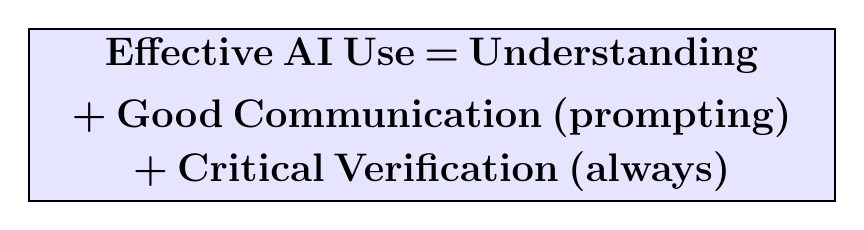
\begin{tikzpicture}
\node[rectangle, draw, thick, text width=10cm, align=center, fill=blue!10] {
    \Large\textbf{Effective AI Use = Understanding}\\[0.3em]
    \Large\textbf{+ Good Communication (prompting)}\\[0.3em]
    \Large\textbf{+ Critical Verification (always)}
};
\end{tikzpicture}
\end{center}

\vspace{1em}

\begin{itemize}
    \item \textbf{Understand:} How they actually work
    \item \textbf{Communicate:} What you really need
    \item \textbf{Verify:} Trust but verify always
\end{itemize}
\end{frame}

\begin{frame}{The Feedback Loop}
\begin{center}
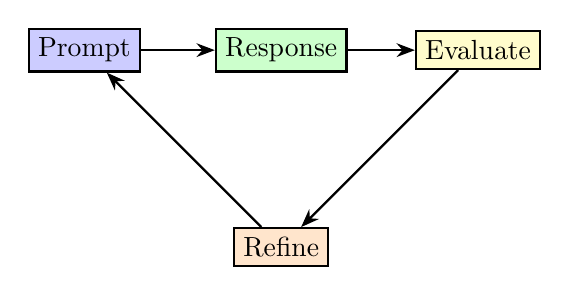
\begin{tikzpicture}[node distance=2.5cm, thick, >=Stealth]
    \node[rectangle, draw, fill=blue!20] (prompt) {Prompt};
    \node[rectangle, draw, fill=green!20, right of=prompt] (response) {Response};
    \node[rectangle, draw, fill=yellow!20, right of=response] (evaluate) {Evaluate};
    \node[rectangle, draw, fill=orange!20, below of=response] (refine) {Refine};

    \draw[->] (prompt) -- (response);
    \draw[->] (response) -- (evaluate);
    \draw[->] (evaluate) -- (refine);
    \draw[->] (refine) -- (prompt);
\end{tikzpicture}
\end{center}

\vspace{1em}

\textbf{Key messages:}
\begin{itemize}
    \item Working with AI is iterative
    \item The skill is making this loop efficient
    \item 2-3 iterations typically gets you to quality
\end{itemize}
\end{frame}

% ===================================================================
% EFFECTIVE PROMPTING SECTION
% ===================================================================

\section{Effective Prompting}

\begin{frame}[fragile]{Four Core Principles: Be Specific}

\textbf{Comparison:}

\begin{columns}[T]
\column{0.48\textwidth}
\textcolor{crosscolor}{\textbf{✗ Less Effective:}}
\begin{lstlisting}
Write a function
to process data
\end{lstlisting}

\column{0.48\textwidth}
\textcolor{checkcolor}{\textbf{✓ More Effective:}}
\begin{lstlisting}
Write a function that
takes user objects and
returns verified
email addresses
\end{lstlisting}
\end{columns}

\vspace{1em}

\begin{exampleblock}{Key Point}
Specificity is about being precise about the outcome, not verbose about the method.
\end{exampleblock}
\end{frame}

\begin{frame}[fragile]{Principles 2-4}

\textbf{Principle 2: Provide Context}

What AI needs:
\begin{itemize}
    \item Relevant code
    \item Constraints (language, framework, style)
    \item Purpose and environment
\end{itemize}

\vspace{0.5em}

\textbf{Principle 3: Show, Don't Tell}
\begin{itemize}
    \item \textcolor{crosscolor}{✗} "Make it follow REST conventions"
    \item \textcolor{checkcolor}{✓} [Show example endpoint] "Create similar for /posts/:id"
\end{itemize}

\vspace{0.5em}

\textbf{Principle 4: Break Down Complex Tasks}
\begin{itemize}
    \item \textcolor{crosscolor}{✗} "Build an authentication system"
    \item \textcolor{checkcolor}{✓} Step 1: Data model $\rightarrow$ Step 2: Password functions $\rightarrow$ Step 3: Login endpoint
\end{itemize}
\end{frame}

\begin{frame}[fragile]{Pattern 1: Structured Request}

\begin{lstlisting}[language=bash, basicstyle=\ttfamily\footnotesize]
## Task
[Clear problem statement]

## Current Code
[Paste code here]

## Requirements
- Specific constraint 1
- Specific constraint 2

## Constraints
- Technology limits
- Style requirements
\end{lstlisting}

\vspace{0.5em}

\begin{exampleblock}{Key Message}
\textbf{Structure creates clarity.} AI (and humans) work better when information is organized.
\end{exampleblock}
\end{frame}

\begin{frame}{Pattern 2: Iterative Refinement}

\textbf{Process flow:}
\begin{center}
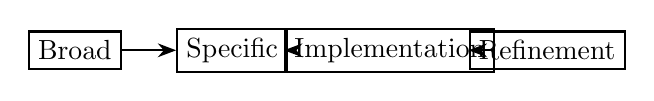
\begin{tikzpicture}[node distance=2cm, thick, >=Stealth]
    \node[rectangle, draw] (broad) {Broad};
    \node[rectangle, draw, right of=broad] (specific) {Specific};
    \node[rectangle, draw, right of=specific] (impl) {Implementation};
    \node[rectangle, draw, right of=impl] (refine) {Refinement};

    \draw[->] (broad) -- (specific);
    \draw[->] (specific) -- (impl);
    \draw[->] (impl) -- (refine);
\end{tikzpicture}
\end{center}

\vspace{1em}

\textbf{Example sequence:}
\begin{enumerate}
    \item "Three approaches to implement caching"
    \item "Expand approach \#2"
    \item "Write the invalidation logic"
\end{enumerate}

\vspace{0.5em}

\textbf{Why it works:}
\begin{itemize}
    \item Each step builds on verified results
    \item Reduces wasted iterations
    \item Lets you course-correct early
\end{itemize}
\end{frame}

\begin{frame}[fragile]{Pattern 3: Rubber Duck}

\textbf{Use case:} Decision making

\vspace{0.5em}

\textbf{Example question:}
\begin{lstlisting}[basicstyle=\ttfamily\footnotesize]
Approach A vs B for permissions:
- A: JSON array on user record
- B: Separate permissions table
- Context: ~10k users, rare changes,
  query on every request
- What tradeoffs should I consider?
\end{lstlisting}

\textbf{Result:} Structured analysis of both options

\vspace{0.5em}

\begin{exampleblock}{Key Point}
You don't need to blindly follow recommendations. Use AI to think through decisions.
\end{exampleblock}
\end{frame}

\begin{frame}{Handling Poor Results}

\textbf{Four strategies when output isn't right:}

\begin{enumerate}
    \item \textbf{Add More Context}\\
    $\rightarrow$ AI might be missing information

    \item \textbf{Provide Negative Examples}\\
    $\rightarrow$ Show what you DON'T want

    \item \textbf{Ask for Alternatives}\\
    $\rightarrow$ "Current approach doesn't work because..."

    \item \textbf{Correct and Continue}\\
    $\rightarrow$ Point out specific issues, ask to fix while keeping rest
\end{enumerate}

\vspace{1em}

\begin{alertblock}{Remember}
Iteration is built-in. 2-3 iterations gets you to quality usually.
\end{alertblock}
\end{frame}

\begin{frame}[fragile]{Anti-Pattern: Prompt Dumping}

\begin{columns}[T]
\column{0.48\textwidth}
\textcolor{crosscolor}{\textbf{✗ DON'T:}}
\begin{lstlisting}[basicstyle=\ttfamily\tiny]
[Entire 10,000 line
 codebase]

"Fix the bug"
\end{lstlisting}

\column{0.48\textwidth}
\textcolor{checkcolor}{\textbf{✓ DO:}}
\begin{lstlisting}[basicstyle=\ttfamily\tiny]
[Identify relevant
 50 lines]

"This throws null
reference when array
is empty.
Add guard clause."
\end{lstlisting}
\end{columns}

\vspace{1em}

\textbf{Why it matters:}
\begin{itemize}
    \item Context pollution degrades output
    \item Harder to iterate
    \item Wastes tokens
\end{itemize}
\end{frame}

% ===================================================================
% CODE INSPECTION SECTION
% ===================================================================

\section{Code Inspection}

\begin{frame}{AI Strengths vs Limitations}

\begin{columns}[T]
\column{0.48\textwidth}
\textbf{\textcolor{checkcolor}{AI STRENGTHS}}
\begin{itemize}
    \item Pattern recognition
    \item Error interpretation
    \item Security patterns
    \item Best practices
    \item Code explanation
\end{itemize}

\column{0.48\textwidth}
\textbf{\textcolor{crosscolor}{AI LIMITATIONS}}
\begin{itemize}
    \item Business logic
    \item Architecture decisions
    \item Your specific context
    \item Historical decisions
    \item Race conditions
\end{itemize}
\end{columns}

\vspace{1em}

\begin{exampleblock}{Key Message}
AI is excellent at mechanical analysis. Human judgment is essential for decisions requiring context.
\end{exampleblock}
\end{frame}

\begin{frame}{Code Review Workflow}

\textbf{Three stages with AI:}

\vspace{0.5em}

\textbf{PRE-COMMIT}
\begin{itemize}
    \item You ask AI to review your own changes
    \item Address obvious issues before human review
    \item Reduces nitpicky back-and-forth
\end{itemize}

\textbf{DURING REVIEW}
\begin{itemize}
    \item Use AI to verify complex logic
    \item Explain unfamiliar patterns
    \item Generate test cases for unclear behavior
\end{itemize}

\textbf{POST-MERGE}
\begin{itemize}
    \item AI helps write release notes
    \item Generates documentation
    \item Updates changelogs
\end{itemize}

\vspace{0.5em}

\textit{Key principle: "AI as first pass, humans for context-dependent decisions"}
\end{frame}

\begin{frame}[fragile]{Review Prompts}

\textbf{Template approach:}

\begin{lstlisting}[basicstyle=\ttfamily\footnotesize]
Review this [type] code for:
- [Specific concerns: security, performance, bugs]
- [Language/framework] best practices

[paste code]
\end{lstlisting}

\vspace{0.5em}

\textbf{Variations:}
\begin{itemize}
    \item \textbf{Comparative:} "Compare these and find differences/issues"
    \item \textbf{Style:} "Review against our conventions: [list]"
    \item \textbf{Focused:} "Security review only"
\end{itemize}

\vspace{0.5em}

\begin{exampleblock}{Key Point}
Focused reviews are more useful than generic ones.
\end{exampleblock}
\end{frame}

\begin{frame}[fragile]{Debugging with AI: Error Interpretation}

\textbf{Template:}

\begin{lstlisting}[basicstyle=\ttfamily\footnotesize]
I'm getting this error:
[error message and stack trace]

Happens when: [trigger]

Relevant code:
[paste code]

Question: What could cause this?
\end{lstlisting}

\vspace{1em}

\textbf{Why this works:}
\begin{itemize}
    \item Structures information
    \item Reduces hallucination
    \item AI generates hypotheses systematically
\end{itemize}
\end{frame}

\begin{frame}{Debugging Techniques}

\begin{center}
\small
\begin{tabular}{ll}
\toprule
\textbf{Technique} & \textbf{When to Use} \\
\midrule
Hypothesis generator & Systematic elimination \\
Rubber duck++ & Validate your theory \\
Trace explainer & Understand execution flow \\
Fix validator & Verify your fix works \\
Comparative debugging & Find subtle differences \\
\bottomrule
\end{tabular}
\end{center}

\vspace{1em}

\textbf{Example:}
\begin{itemize}
    \item "Why works: [code A]"
    \item "Why doesn't: [code B]"
\end{itemize}

\textit{Result: Focused analysis of differences}
\end{frame}

\begin{frame}{Debugging Workflow}

\textbf{Three phases:}

\vspace{0.5em}

\begin{columns}[T]
\column{0.32\textwidth}
\textbf{BEFORE ASKING AI}
\begin{itemize}
    \item[\checkmark] Exact errors
    \item[\checkmark] Repro steps
    \item[\checkmark] Relevant code
    \item[\checkmark] Recent changes
    \item[\checkmark] Environment
\end{itemize}

\column{0.32\textwidth}
\textbf{START BROAD}
\begin{itemize}
    \item Initial hypotheses
    \item Most likely first
    \item Share findings
    \item Iterate \& narrow
\end{itemize}

\column{0.32\textwidth}
\textbf{VERIFY FIXES}
\begin{itemize}
    \item Understand why
    \item Side effects?
    \item Test edge cases
    \item Don't blindly apply
\end{itemize}
\end{columns}
\end{frame}

% ===================================================================
% AUTOMATION SECTION
% ===================================================================

\section{Automation}

\begin{frame}{Core Principle: Augment, Don't Replace}

\begin{center}
\Large
\textbf{Augment, Don't Replace}
\end{center}

\vspace{0.5em}

\small
\textit{AI automation works best when enhancing existing processes,\\not replacing critical checks}

\vspace{1em}

\begin{center}
\footnotesize
\begin{tabular}{ll}
\toprule
\textbf{USE AI AUTOMATION FOR} & \textbf{AVOID FOR} \\
\midrule
Variable inputs (code review, docs) & Deterministic ops (tests, deploys) \\
Pattern recognition (vulnerabilities) & High-stakes decisions (prod approvals) \\
Natural language (messages) & Guaranteed correctness (security) \\
\bottomrule
\end{tabular}
\end{center}
\end{frame}

\begin{frame}{Three Essential Patterns}

\textbf{Pattern 1: Generate and Review}
\begin{itemize}
    \item AI generates (PR descriptions, fixes, notes)
    \item Human reviews
    \item System applies
\end{itemize}

\vspace{0.5em}

\textbf{Pattern 2: Triage and Route}
\begin{itemize}
    \item AI classifies (labels, categorization)
    \item System routes appropriately
    \item Humans handle with better context
\end{itemize}

\vspace{0.5em}

\textbf{Pattern 3: Augment and Assist}
\begin{itemize}
    \item Human works
    \item AI suggests in real-time
    \item Human decides what to accept
\end{itemize}
\end{frame}

\begin{frame}{CI/CD Integration Points}

\begin{center}
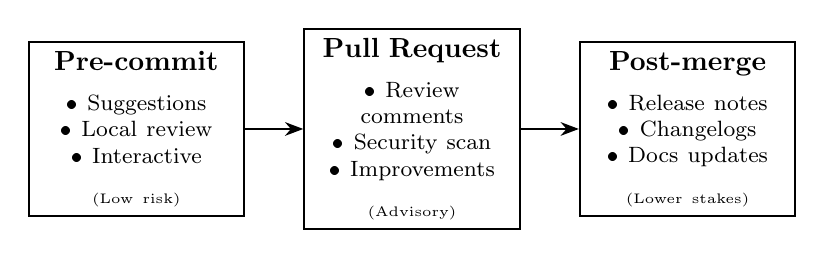
\begin{tikzpicture}[node distance=3.5cm, thick, >=Stealth]
    \node[rectangle, draw, text width=2.5cm, align=center] (pre) {
        \textbf{Pre-commit}\\[0.5em]
        \footnotesize
        • Suggestions\\
        • Local review\\
        • Interactive\\[0.3em]
        \tiny (Low risk)
    };

    \node[rectangle, draw, text width=2.5cm, align=center, right of=pre] (pr) {
        \textbf{Pull Request}\\[0.5em]
        \footnotesize
        • Review comments\\
        • Security scan\\
        • Improvements\\[0.3em]
        \tiny (Advisory)
    };

    \node[rectangle, draw, text width=2.5cm, align=center, right of=pr] (post) {
        \textbf{Post-merge}\\[0.5em]
        \footnotesize
        • Release notes\\
        • Changelogs\\
        • Docs updates\\[0.3em]
        \tiny (Lower stakes)
    };

    \draw[->] (pre) -- (pr);
    \draw[->] (pr) -- (post);
\end{tikzpicture}
\end{center}

\vspace{1em}

\begin{exampleblock}{Key Principle}
Each stage has different risk/benefit tradeoffs.
\end{exampleblock}
\end{frame}

\begin{frame}{Pipeline Considerations}

\textbf{Three critical factors:}

\vspace{0.5em}

\textbf{FAIL-SAFE DESIGN}
\begin{itemize}
    \item Don't break pipelines on AI failures
    \item Make AI steps optional
    \item Set reasonable timeouts
\end{itemize}

\textbf{COST CONTROL}
\begin{itemize}
    \item Limit to key branches
    \item Skip draft PRs
    \item Cache results, monitor spend
\end{itemize}

\textbf{OBSERVABILITY}
\begin{itemize}
    \item Log decisions and track metrics
    \item Monitor false positive rate
    \item Track developer override rate
\end{itemize}
\end{frame}

\begin{frame}{Security \& Data}

\textbf{Key considerations:}

\vspace{0.5em}

\textbf{DATA EXPOSURE}
\begin{itemize}
    \item What goes to AI services?
    \item May be logged or used for training
    \item Filter sensitive files, redact secrets
\end{itemize}

\textbf{SUPPLY CHAIN RISK}
\begin{itemize}
    \item AI suggestions should be reviewed
    \item Don't auto-apply changes
    \item Maintain generate-and-review pattern
\end{itemize}

\textbf{FEEDBACK LOOPS}
\begin{itemize}
    \item Record dismissals
    \item Use data to improve prompts
    \item Monitor false positive rate $\rightarrow$ maintain trust
\end{itemize}
\end{frame}

% ===================================================================
% SECURITY SECTION
% ===================================================================

\section{Security}

\begin{frame}{Threat Categories}

\textbf{Three layers of security:}

\vspace{0.5em}

\begin{columns}[T]
\column{0.32\textwidth}
\textbf{APPLICATION}
\begin{itemize}
    \item Authorization
    \item Access control
    \item Business logic
\end{itemize}

\column{0.32\textwidth}
\textbf{AI LAYER}\\
\textit{(focus of session)}
\begin{itemize}
    \item Prompt injection
    \item Output manipulation
    \item Data exposure
\end{itemize}

\column{0.32\textwidth}
\textbf{INFRASTRUCTURE}
\begin{itemize}
    \item API security
    \item Data storage
    \item Network security
\end{itemize}
\end{columns}
\end{frame}

\begin{frame}{Key Threat: Prompt Injection}

\begin{alertblock}{Warning}
\textbf{No complete solution exists.} Goal: reduce risk and limit impact.
\end{alertblock}

\vspace{0.5em}

\textbf{How it works:}
\begin{center}
\textit{User input + Instructions}\\
\small(AI can't reliably distinguish between them)
\end{center}

\vspace{0.5em}

\textbf{Attack types:}
\begin{enumerate}
    \item \textbf{Direct injection} - Attack payload in user input
    \item \textbf{Indirect injection} - Attack hidden in processed data
    \item \textbf{Jailbreaking} - Roleplay attacks to bypass safety guidelines
\end{enumerate}

\vspace{0.5em}

\textbf{Mitigation:} Defense in depth (multiple layers)
\end{frame}

\begin{frame}{Defense in Depth Approach}

\begin{center}
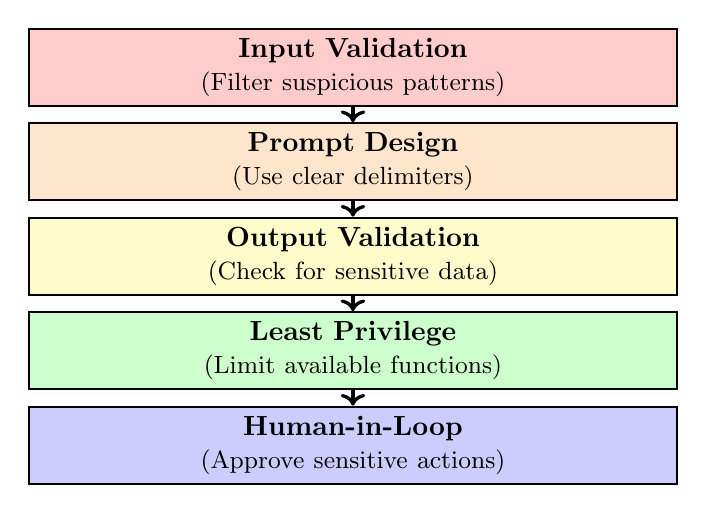
\begin{tikzpicture}[node distance=1.2cm, thick]
    \node[rectangle, draw, text width=8cm, align=center, fill=red!20] (input) {
        \textbf{Input Validation}\\
        \small (Filter suspicious patterns)
    };
    \node[rectangle, draw, text width=8cm, align=center, fill=orange!20, below of=input] (prompt) {
        \textbf{Prompt Design}\\
        \small (Use clear delimiters)
    };
    \node[rectangle, draw, text width=8cm, align=center, fill=yellow!20, below of=prompt] (output) {
        \textbf{Output Validation}\\
        \small (Check for sensitive data)
    };
    \node[rectangle, draw, text width=8cm, align=center, fill=green!20, below of=output] (privilege) {
        \textbf{Least Privilege}\\
        \small (Limit available functions)
    };
    \node[rectangle, draw, text width=8cm, align=center, fill=blue!20, below of=privilege] (human) {
        \textbf{Human-in-Loop}\\
        \small (Approve sensitive actions)
    };

    \draw[->, very thick] (input) -- (prompt);
    \draw[->, very thick] (prompt) -- (output);
    \draw[->, very thick] (output) -- (privilege);
    \draw[->, very thick] (privilege) -- (human);
\end{tikzpicture}
\end{center}

\vspace{0.5em}

\textbf{Key:} Multiple layers, not single solution
\end{frame}

\begin{frame}{Practical Guidance}

\begin{columns}[T]
\column{0.48\textwidth}
\textbf{\textcolor{checkcolor}{DO:}}
\begin{itemize}
    \item[\checkmark] Review generated code carefully
    \item[\checkmark] Watch for security anti-patterns
    \item[\checkmark] Use .gitignore for sensitive files
    \item[\checkmark] Redact sensitive data in prompts
    \item[\checkmark] Consult security team
\end{itemize}

\column{0.48\textwidth}
\textbf{\textcolor{crosscolor}{DON'T:}}
\begin{itemize}
    \item[✗] Blindly accept suggestions
    \item[✗] Paste production credentials
    \item[✗] Assume AI knows your threat model
    \item[✗] Use AI alone for security decisions
\end{itemize}
\end{columns}

\vspace{1em}

\textbf{Common patterns to watch:}
\begin{itemize}
    \item SQL concatenation vs parameterized queries
    \item Missing input validation
    \item Overly broad exception handling
    \item Hardcoded credentials
\end{itemize}
\end{frame}

% ===================================================================
% TRANSITION TO DEMO
% ===================================================================

\section{Demo}

\begin{frame}{What We Just Covered}

\begin{center}
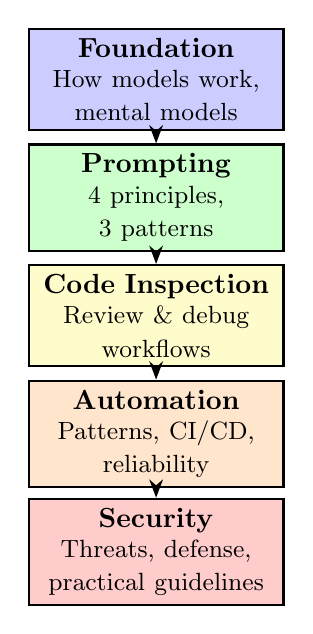
\begin{tikzpicture}[node distance=1.5cm, thick, >=Stealth]
    \node[rectangle, draw, fill=blue!20, text width=3cm, align=center] (found) {
        \textbf{Foundation}\\
        \small How models work,\\mental models
    };
    \node[rectangle, draw, fill=green!20, text width=3cm, align=center, below of=found] (prompt) {
        \textbf{Prompting}\\
        \small 4 principles,\\3 patterns
    };
    \node[rectangle, draw, fill=yellow!20, text width=3cm, align=center, below of=prompt] (code) {
        \textbf{Code Inspection}\\
        \small Review \& debug\\workflows
    };
    \node[rectangle, draw, fill=orange!20, text width=3cm, align=center, below of=code] (auto) {
        \textbf{Automation}\\
        \small Patterns, CI/CD,\\reliability
    };
    \node[rectangle, draw, fill=red!20, text width=3cm, align=center, below of=auto] (sec) {
        \textbf{Security}\\
        \small Threats, defense,\\practical guidelines
    };

    \draw[->] (found) -- (prompt);
    \draw[->] (prompt) -- (code);
    \draw[->] (code) -- (auto);
    \draw[->] (auto) -- (sec);
\end{tikzpicture}
\end{center}
\end{frame}

\begin{frame}{Let's See It In Practice}

\Large
\textit{"Let's see how these principles apply in practice."}

\vspace{1em}

\normalsize
\textbf{We'll do a live walkthrough of:}

\begin{enumerate}
    \item Effective prompting in action
    \item Code review and debugging workflow
    \item How to use these tools day-to-day
\end{enumerate}

\vspace{2em}

\begin{center}
\large
\textbf{Questions are always welcome}\\
\normalsize
Either now or after the demo
\end{center}
\end{frame}

% ===================================================================
% BACKUP SLIDES (Optional)
% ===================================================================

\appendix

\begin{frame}[plain]
\begin{center}
\Huge Thank You!

\vspace{2em}

\Large Questions?
\end{center}
\end{frame}

\end{document}
